\documentclass[aspectratio=168]{beamer}

\newif\ifwhite
\whitetrue
% %%%%%%%%%%%%%%%%%%%%%%%%%%%%%%%%%%%%%%%%%%%%%%%%%%%
% %%%%%%%%%%%%%%%%%%%%%%%%%%%%%%%%%%%%%%%%%%%%%%%%%%%
% PATH to the beamer-templates-v3 folder
\def\cspath{../../../../../../Latex-workspace/}
% %%%%%%%%%%%%%%%%%%%%%%%%%%%%%%%%%%%%%%%%%%%%%%%%%%%
% %%%%%%%%%%%%%%%%%%%%%%%%%%%%%%%%%%%%%%%%%%%%%%%%%%%
% Main declarations for this slides
\usepackage{\cspath beamer-templates-v3/theme}
\usetikzlibrary{shapes,arrows.meta}
\usetikzlibrary{arrows.meta}
\usetikzlibrary{shapes,snakes}
\usetikzlibrary{shapes}
\usetikzlibrary{decorations.pathreplacing}
\usetikzlibrary{arrows,automata,positioning}
\usetikzlibrary{shapes.symbols}
\usetikzlibrary{arrows.meta}
\usetikzlibrary{shapes,snakes}

\setbeamersize{text margin left=0cm}
\setbeamersize{text margin right=0cm}

\def\csminilogo{\cspath beamer-templates-v3/Figs/CentraleSupelec-Logo-V-color.png}
% %%%%%%%%%%%%%%%%%%%%%%%%%%%%%%%%%%%%%%%%%%%%%%%%%%%
% %%%%%%%%%%%%%%%%%%%%%%%%%%%%%%%%%%%%%%%%%%%%%%%%%%%
% The main document 
\begin{document}    
% %%%%%%%%%%%%%%%%%%%%%%%%%%%%%%%%%%%%%%%%%%%%%%%%%%%
% %%%%%%%%%%%%%%%%%%%%%%%%%%%%%%%%%%%%%%%%%%%%%%%%%%%
\begin{frame}[plain]

\begin{center}
\begin{tikzpicture}[->,>=stealth',shorten >=1pt,auto,node distance=2.8cm, semithick]
\tikzstyle{every state}=[fill=red,draw=none,text=white]
  
\only<1>{
\node[initial,state] (A)                    {\bf s1, I};
\node[state]         (B) [right of=A] {\bf s2, I};
\node[state]         (C) [right of=B] {\bf s3, I};}

\only<2->{
\node[initial,state] (A)                    {\bf s1', J};
\node[state]         (B) [right of=A] {\bf s2', J};}

\only<2->{\node[state]         (C) [right of=B] {\bf s3', J};}

\only<1->{\path (A) edge     [bend left]         node {ev1} (B);}
\only<1,2>{\path (B) edge     [bend left]         node {ev2} (C);}

\onslide<3>{
\node[state]         (C1) [below of=B] {\bf s31, J};
\node[state]         (C2) [below of=C] {\bf s32, J};
\path (B) edge     [bend right]         node {ev21} (C1);
\path (C1) edge     [bend right]         node {ev22} (C2);
\path (C2) edge     [bend left]         node {ev2} (C);
}
\end{tikzpicture}
\end{center}

\end{frame}
% %%%%%%%%%%%%%%%%%%%%%%%%%%%%%%%%%%%%%%%%%%%%%%%%%%%
% %%%%%%%%%%%%%%%%%%%%%%%%%%%%%%%%%%%%%%%%%%%%%%%%%%% 
\end{document}
% %%%%%%%%%%%%%%%%%%%%%%%%%%%%%%%%%%%%%%%%%%%%%%%%%%%
% %%%%%%%%%%%%%%%%%%%%%%%%%%%%%%%%%%%%%%%%%%%%%%%%%%%
